\documentclass[a4paper,12pt]{report}
\usepackage[portuguese]{babel}
\usepackage{indentfirst}
\usepackage[T1]{fontenc}
\usepackage[utf8]{inputenc}
\usepackage{csquotes}
\usepackage{array}
\usepackage[font={footnotesize,it}]{caption}
\usepackage{graphicx} 
\usepackage{float}
\usepackage{color, colortbl}
\usepackage{titlesec}
\usepackage{longtable}
\usepackage{pdfpages} 
\graphicspath{ {./supportFiles/}}
\usepackage{tabularx}
\setlength{\parskip}{\baselineskip}
%\usepackage{lmodern} 

%\usepackage[top=2.5cm, bottom=2.5cm, left=3cm, right=2.5cm]{geometry}

\begin{document}
	
	\begin{titlepage}
		\begin{center}
		
		\begin{figure}[H]
		\begin{center}
			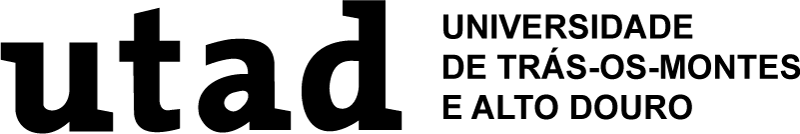
\includegraphics[scale=0.45]{logo_utad_completo_preto}	
		\end{center}
		\label{fig:logoUTAD}	
		\end{figure}
		
		\vspace{3cm}
		\huge
		\textbf{FoodFinder}
		
		%\vspace{0.5cm}
		\Large
		Design e Desenvolvimento de uma Aplicação Web\\
		Etapa 1
		
		
		\vspace{2.5cm}
		\large
		David Ferreira, 68222\\
		André Mendes, 68228\\
		João Santos, 68943\\
		Diogo Mesquita, 69185\\
		
		\vspace{2.5cm}
		Licenciatura em Engenharia Informática\\
		Laboratório de Aplicações Web e Base de Dados \\
		
		\vspace{1.5cm}		
		Vila Real, novembro de 2020
		
		\end{center}
	\end{titlepage}	
	
	
	
	
	
%--------------------------------------------------------------
	
	\pagenumbering{roman}
	
	\begin{abstract}
	Atualmente, as aplicações \textit{Web} estão em todo o lado e esta é uma tendência que continua a aumentar com cada vez mais plataformas, ferramentas e informação a transitar para serviços remotos. Desta maneira, este tipo de aplicação faz, cada vez mais, parte do nosso dia-a-dia e ocupam um espaço importante na vida das organizações.
	
	Com o intuito de proceder ao \textit{design} e implementação de uma aplicação \textit{Web} que consiste, entre várias funcionalidades, num portal de restaurantes e dos seus pratos do dia, o presente documento dedica-se a explorar e apresentar o modelo conceptual de dados, a análise dos requisitos funcionais e a consequente especificação dos casos de uso do sistema. Este é um passo imprescindível no planeamento desta \textit{web app} de modo a garantir que a solução final responda corretamente às necessidades do sistema a construir.
	
	\end{abstract}	
	
	
	\newpage
	\tableofcontents
	
	\pagenumbering{arabic}
	\newpage	
	
%--------------------------------------------------------------	
\chapter{Introdução}	

	Uma aplicação \textit{web} permite que o processamento de informação seja instanciado remotamente através de um \textit{browser} e executado parcialmente num servidor \textit{web}, servidor aplicacional (\textit{application server}) e/ou num servidor de base de dados (\textit{database server}) (Bruno \& Thom, 2005). O surgimento deste tipo de tecnologias permitiu que uma aplicação tivesse um maior número de utilizadores, que estes estivessem dispersos pelo mundo e que existisse uma forma mais fácil para compartilhar informação entre diferentes utilizadores e diferentes dispositivos.
	
	Desse modo, o estudo deste tipo de plataformas e tecnologias - tanto a nível de planeamento, \textit{design} e implementação - afigura-se como um elemento crucial na atualidade.
	
	Com esse intuito, vamos realizar o planeamento, \textit{design} e implementação de uma aplicação \textit{web} que se baseia num portal onde é possível a restaurantes registados inserirem informação sobre o seu estabelecimento e adicionarem os seus pratos do dia. Por outro lado, clientes autenticados deverão ter a capacidade de guardar restaurantes e pratos do dia na sua lista de favoritos.  
	
	Para isso, esse desenvolvimento será dividido em três fases distintas, mas cada uma necessária para a fase consequente. Este presente documento dedica-se a apresentar e a explorar a primeira fase deste projeto. Desse modo, em primeiro lugar,  este começa por estabelecer as classes de utilizadores do sistema e, em seguida, o modelo conceptual dos dados, a análise e levantamento dos requisitos do sistema a construir e, por fim, os casos de uso através da sua representação com o diagrama de casos-de-uso da família UML.
	
	
%--------------------------------------------------------------
\chapter{Classes de Utilizadores do Sistema}	

	Neste capítulo, são apresentadas na tabela \ref{tab:classesUtilizadores} as diferentes classes de utilizadores que irão interagir com o sistema em estudo, tal como uma breve descrição das funcionalidades às quais cada classe tem acesso.
	
	\begin{table}[H]
	\begin{tabularx}{\textwidth}{|l|X|}
	\hline
	Classe de Utilizador & Descrição\\ 
	\hline
 	\hline
 	Administrador & Responsável por criar outros utilizadores administradores, aceitar pedidos de registo de restaurantes e fazer a gestão de utilizadores.\\
 	\hline 
	Visitante & É um utilizador não autenticado. Tem acesso a funcionalidades básicas como consultar informação dos restaurantes e consultar os seus pratos do dia.\\ 
	\hline
	Cliente & Para além de compartilhar as funcionalidades do utilizador Visitante, ainda pode pesquisar pratos do dia por palavra-chave ou tipo, tal como adicionar pratos e restaurantes à sua lista de favoritos.\\
	\hline
	Restaurante & Para além de compartilhar as funcionalidades do utilizador Visitante, pode, também, fazer a gestão dos seus pratos do dia.\\
	\hline
	\end{tabularx}
	\caption{As diferentes classes de utilizador do sistema.}
	\label{tab:classesUtilizadores}
	\end{table}	
	
	
	
	


%--------------------------------------------------------------
\chapter{Modelo Conceptual dos Dados}

	O modelo entidade-relacionamento é utilizado para descrever níveis externos e conceituais de dados e são independentes dos aspetos físicos e internos. São úteis, pois para além de apresentarem o que deverá estar presente na base de dados, eles também fornecem vários outros detalhes como a representação explícita de objetos, atributos, relações, constrangimentos e outros (Ricardo \& Urban, 2017).
	
	No diagrama \ref{fig:diagramaER} é apresentado o diagrama entidade-relacionamento para o sistema FoodFinder. Analisando o mesmo, podemos, rapidamente, identificar quais são as entidades, e as suas propriedades, que irão estar patentes na nossa base de dados: numa primeira análise, estas serão Utilizador, Restaurante, Cliente, Administrador, Prato\_do\_Dia e Destaque. Por outro lado, também podemos perceber as relações que estas entidades estabelecem entre si.

	\begin{figure}[H]
	\begin{center}
	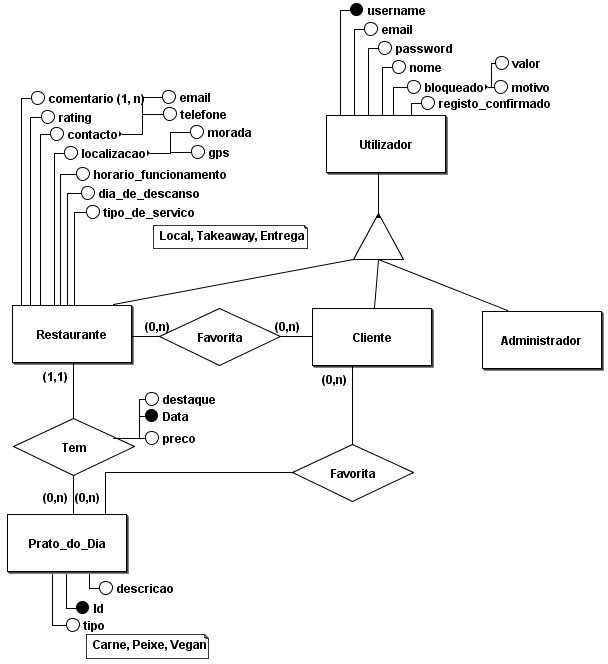
\includegraphics[scale=0.85]{diagramaER}	
	\end{center}
	\medskip
	\caption{O modelo conceptual dos dados do sistema FoodFinder, através de um diagrama E-R.}
	\label{fig:diagramaER}	
	\end{figure}

%--------------------------------------------------------------
\chapter{Análise e Levantamento dos Requisitos Funcionais}	

	Segundo Sommerville \& Sawyer, os requisitos são a especificação do que deverá ser implementado (Sommerville \& Sawyer, 2006). No caso dos requisitos funcionais, estes são descrições do que os desenvolvedores deverão implementar para permitir que os utilizadores executem as suas tarefas de acordo com os objetivos e o intuito do sistema. 

	Bell, Morrey \& Pugh afirmam mesmo que o estabelecimento e a definição dos requisitos é a atividade isolada mais importante no desenvolvimento de \textit{software}, pois se não fomos capaz de corretamente especificar o que é preciso, é inútil implementa-lo (Bell, Morrey \& Pugh, 1992).
	
	Desse modo, em seguida, são apresentados os requisitos funcionais que deverão ser implementados na construção do sistema em estudo.
	
\begin{enumerate}
\item O sistema FoodFinder deverá permitir o registo dos clientes.
\item O sistema FoodFinder deverá permitir o registo dos restaurantes.
\item O sistema FoodFinder deverá permitir a criação de Administradores.
\item O sistema FoodFinder deverá permitir a inserção de informação do utilizador.
\item O sistema FoodFinder deverá enviar uma mensagem para confirmação do registo do cliente.
\item O sistema FoodFinder deverá permitir aceitar pedidos de registo de restaurantes.
\item O sistema FoodFinder deverá permitir o bloqueio dos utilizadores.
\item O sistema FoodFinder deverá permitir a autenticação do utilizador.
\item O sistema FoodFinder deverá informar motivo do bloqueio a quando autenticação.
\item O sistema FoodFinder deverá permitir realizar a gestão dos utilizadores.
\bigskip
\bigskip
\bigskip
\item O sistema FoodFinder deverá permitir a inserção de um prato do dia.
\item O sistema FoodFinder deverá manter um histórico dos pratos inseridos.
\item O sistema FoodFinder deverá permitir reutilizar pratos anteriores.
\item O sistema FoodFinder deverá permitir adicionar prato aos destaques do sistema.
\bigskip
\bigskip
\bigskip
\item O sistema FoodFinder deverá permitir a consulta de pratos do dia.
\item O sistema FoodFinder deverá permitir a consulta de restaurantes.
\item O sistema FoodFinder deverá permitir pesquisar um restaurante através de proximidades geográficas.
\item O sistema FoodFinder deverá permitir pesquisar um prato do dia por \textit{keyword}.
\item O sistema FoodFinder deverá permitir adicionar à lista de favoritos um prato do dia.
\item O sistema FoodFinder deverá permitir adicionar à lista de favoritos um restaurante.
\item O sistema FoodFinder deverá enviar notificação quando prato do dia favorito encontra-se disponível.
\item O sistema FoodFinder deverá permitir avaliar um restaurante.
\end{enumerate}


%--------------------------------------------------------------
\chapter{Os Casos-de-Uso}	

	Os casos de uso são as técnicas para capturar os requisitos funcionais de um sistema, descrevendo as interações típicas entre os utilizadores de um sistema e o próprio sistema (Fowler, 2004).

	Assim, com base nos requisitos que foram anteriormente apresentados, no diagrama \ref{fig:casoUso_comum} estão representados os casos-de-uso que são comuns aos diferentes atores do sistema. Por outro lado, nos diagramas \ref{fig:casoUso_cliente}, \ref{fig:casoUso_comum}, \ref{fig:casoUso_restaurante} são apresentados os casos-de-uso específicos e particulares a cada um dos atores.
	
	
	\begin{figure}[H]
	\begin{center}
	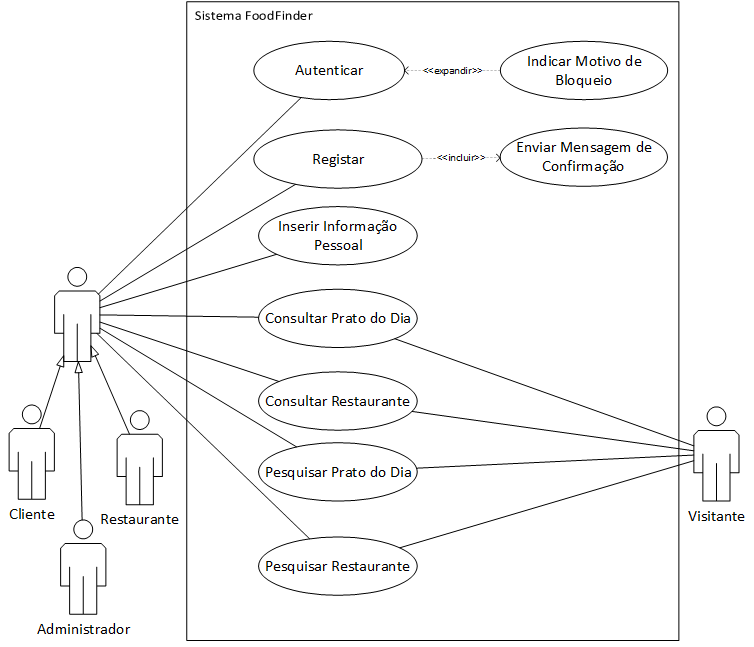
\includegraphics[scale=0.68]{casoUso_comum}	
	\end{center}
	\medskip
	\caption{Diagrama que apresenta os casos-de-uso comuns aos vários atores do sistema FoodFinder.}
	\label{fig:casoUso_comum}	
	\end{figure}
	
	\begin{figure}[H]
	\begin{center}
	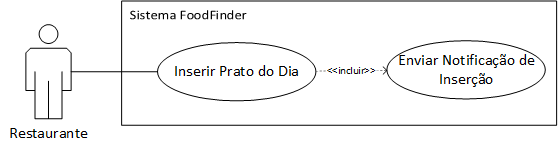
\includegraphics[scale=0.70]{casoUso_restaurante}	
	\end{center}
	\medskip
	\caption{O diagrama dos casos-de-uso do sistema FoodFinder relativos ao ator Restaurante.}
	\label{fig:casoUso_restaurante}	
	\end{figure}
	
	\begin{figure}[H]
	\begin{center}
	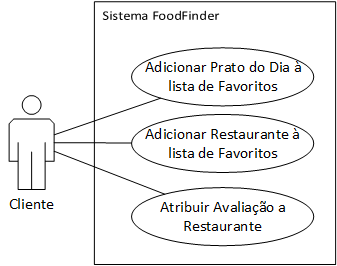
\includegraphics[scale=0.70]{casoUso_cliente}	
	\end{center}
	\medskip
	\caption{O diagrama dos casos-de-uso do sistema FoodFinder relativos ao ator Cliente.}
	\label{fig:casoUso_cliente}	
	\end{figure}	
	
	\begin{figure}[H]
	\begin{center}
	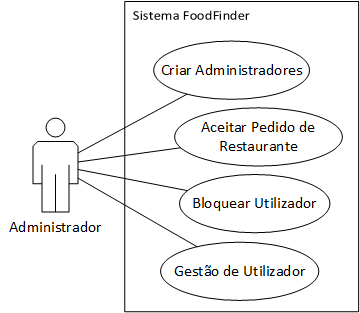
\includegraphics[scale=0.70]{casoUso_administrador}	
	\end{center}
	\medskip
	\caption{O diagrama dos casos-de-uso do sistema FoodFinder relativos ao ator Administrador.}
	\label{fig:casoUso_administrador}	
	\end{figure}
	

%--------------------------------------------------------------
\chapter{Conclusão}	

	O grande crescimento no uso de aplicações \textit{web} e o aumento da sua complexidade exige que mais atenções sejam feitas no que toca ao seu planeamento e \textit{design}.
	
	O estudo desenvolvido nesta fase do trabalho prático, permitiu construir as bases nas quais sustentarão o planeamento adicional e a própria implementação do sistema a construir. Com o modelo conceptual dos dados temos uma primeira visão sobre a base de dados que suportará o sistema, incluindo as entidades e relações que dela farão parte. Com o levantamento e análise de requisitos, tal como a construção e definição dos casos-de-uso, temos uma boa descrição para os diferentes utilizadores que farão uso do sistema e de que forma eles interagirão com ele. 
	
	A próxima fase residirá no mapeamento do modelo concetual dos dados para o modelo relacional e a consequente implementação do modelo físico da base de dados. Da mesma forma, também serão especificadas as interfaces de \textit{backoffice} e \textit{frontoffice} recorrendo a \textit{mockups}.

%--------------------------------------------------------	
\titleformat{\chapter}[display]
{\normalfont\bfseries}{}{0pt}{\Huge}
\chapter{Referências}

Bell, D., Morrey, I. \& Pugh, J. (2006). Software Engineering: A programming approach. Prentice Hall.

Bruno, V. \& Thom, J. (2005). Characteristics of Web applications that affect usability: A review. 

Fowler, M. (2004). UML Destilled: a brief guide to the standard object modeling language. Addison-Wesley Professional.

Ricardo, C. M., \& Urban, S. D. (2017). Database Processing: Fundamentals, Design and Implementation. Pearson.

Sommerville, I. \& Sawyer, P. (2006). Requirements Engineering: a good Practice Guide. John Wiley.


	
\end{document}